\documentclass[11pt]{article}
\usepackage[english]{babel}
\usepackage{minted}
\usepackage{graphicx}
\usepackage{float}
\usepackage{xcolor}
\usepackage[left=25mm, top=25mm, bottom=30mm, right=25mm]{geometry}
\usepackage[colorlinks=true, linkcolor=blue, urlcolor=cyan]{hyperref}

\renewcommand\thesubsection{\thesection.\alph{subsection}}
\renewcommand\thesubsubsection{\thesubsection.\roman{subsubsection}}

\graphicspath{{./figures/}}
\definecolor{mintedbg}{rgb}{0.98,0.97,0.93}

\title{COL334: Assignment 1}
\author{Sayam Sethi}
\date{August 2021}

\begin{document}

\maketitle

\tableofcontents

\section{Networking Tools}

\subsection{Local IP Address}
To obtain the \textit{IP address} of a device, running \texttt{ifconfig} gives the detailed information about the same.

\subsubsection{Router}
The following output is obtained on running the command when connected to Wi-Fi router:
\begin{figure}[H]
    \centering
    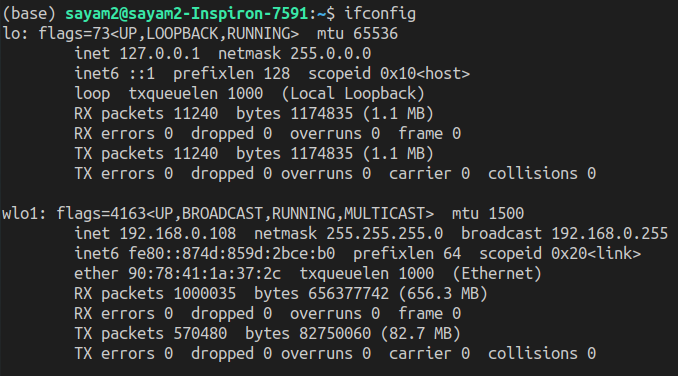
\includegraphics[width=0.5\textwidth]{ifconfig_router.png}
    \caption{\texttt{ifconfig} on router}
\end{figure}
The first entry in the output, i.e., \texttt{lo}, is the \textbf{loopback connection} which is used to connect to ports on the same device.\par
The second entry, \texttt{wlo1}, is the relevant one and it contains information about the \textbf{Wi-Fi connection}. The \textit{IP address} is the \texttt{inet} address: $192.168.0.108$.

\subsubsection{Mobile Hotspot}
On connecting to mobile hotspot, following is the output of \texttt{ifconfig}:
\begin{figure}[H]
    \centering
    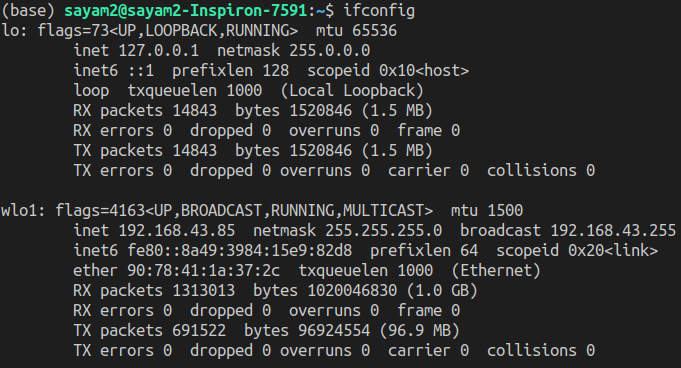
\includegraphics[width=0.5\textwidth]{ifconfig_hotspot.png}
    \caption{\texttt{ifconfig} on mobile hotspot}
\end{figure}
The \textit{IP address} which is the \texttt{inet} address now has changed to: $192.168.43.85$.


\subsection{IP Address of Different Servers}
To obtain the \textit{IP address} of servers, the \texttt{nslookup} command is used. This \textit{IP address} depends on the \textbf{DNS server} being used.

\subsubsection{\href{https://www.google.com}{Google}}
\begin{figure}[H]
    \centering
    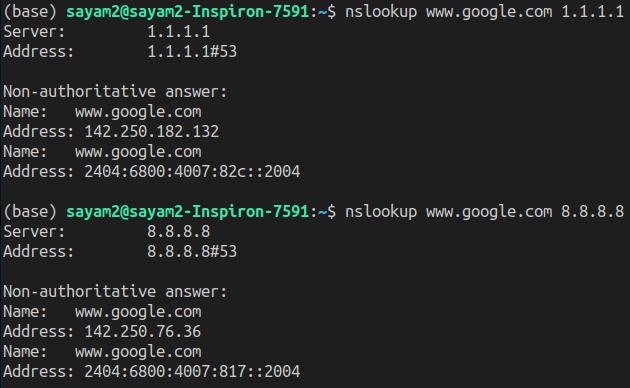
\includegraphics[width=0.5\textwidth]{nslookup_google.png}
    \caption{\texttt{nslookup} for \href{https://www.google.com}{Google} using $2$ different DNS servers}
\end{figure}
Using \textbf{Cloudfare 1.1.1.1 DNS} server gave the \textit{IP address} as $142.250.182.132$, while using \textbf{Google Public DNS} server resulted in an \textit{IP address} of $142.250.76.36$.

\subsubsection{\href{https://www.facebook.com}{Facebook}}
\begin{figure}[H]
    \centering
    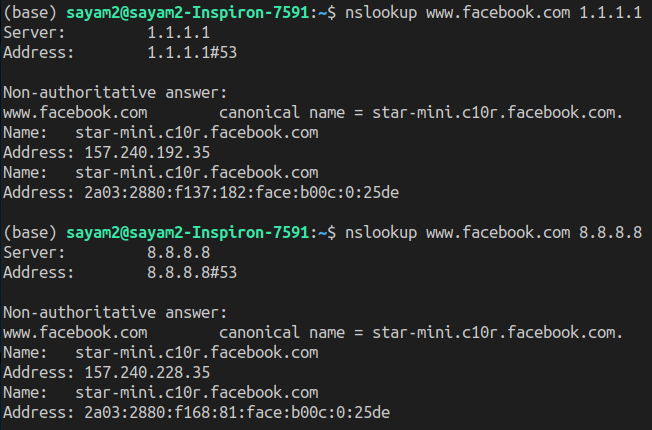
\includegraphics[width=0.5\textwidth]{nslookup_facebook.png}
    \caption{\texttt{nslookup} for \href{https://www.facebook.com}{Facebook} using $2$ different DNS servers}
\end{figure}
Using \textbf{Cloudfare 1.1.1.1 DNS} server gave the \textit{IP address} as $157.240.192.35$, while using \textbf{Google Public DNS} server resulted in an \textit{IP address} of $157.240.228.35$.


\subsection{Ping (Pong)}
To analyse the ping values, a script was written to \textbf{binary search} on different values of \textit{packet size} and \textit{TTL value}.\par
The size of the transmitted packet is always $28$ bytes larger than the size set using the \texttt{-s} command. This is the header data which has the same structure for all packets.

\subsubsection{Packet Size}

\paragraph{\href{https://www.iitd.ac.in}{IITD}} The maximum packet size that can be pinged is $29116\ (+28)$ bytes.
\paragraph{\href{https://www.google.com}{Google}} The maximum pingable packet size is only $68\ (+28)$ bytes.
\paragraph{\href{https://www.facebook.com}{Facebook}} The maximum packet size that is pinged is $1452\ (+28)$ bytes.

\subsubsection{Time To Live (TTL) Value}

\paragraph{\href{https://www.iitd.ac.in}{IITD}} The smallest TTL value achieved is $12$ hops.
\paragraph{\href{https://www.google.com}{Google}} The least number of hops taken to ping Google is $8$ hops.
\paragraph{\href{https://www.facebook.com}{Facebook}} Facebook is reached within atleast $10$ hops.


\subsection{\texttt{traceroute}}

\subsubsection{\href{https://www.iitd.ac.in}{IITD}}
\paragraph{Router} Running \texttt{traceroute} to \href{https://www.iitd.ac.in}{IITD} using router gave no response:
\inputminted[bgcolor=mintedbg]{text}{outputs/traceroute_iitd_novpn}

\paragraph{Router + VPN} Running \texttt{traceroute} using \textit{IITD VPN} was successful and gave the following trace:
\inputminted[bgcolor=mintedbg]{text}{outputs/traceroute_iitd_vpn}

\subsubsection{\href{https://www.google.com}{Google}}

\paragraph{Router} The trace obtained was:
\inputminted[bgcolor=mintedbg]{text}{outputs/traceroute_google_router}

\paragraph{Mobile Hotspot} The trace now obtained was:
\inputminted[bgcolor=mintedbg]{text}{outputs/traceroute_google_hotspot}

\subsubsection{Observations}
The following observations were made when running \texttt{traceroute}:
\begin{enumerate}
    \item Three packets are pinged for each hop value to \textit{display consistency, or a lack thereof, in the route}
    \item The router at the second hop value doesn't ping when using the default (no additional options) \texttt{traceroute} command
    \item Different routes are followed when using different networks to access the same URL
\end{enumerate}

\subsubsection{Changes to Improve Tracing}
\begin{enumerate}
    \item Traceroute by default uses \textbf{UDP} which is unreliable and hence many servers do not respond to it. To avoid this issue, \texttt{-I} flag can be used, which uses \textbf{ICPM echo} as the packet instead.
        \begin{figure}[H]
            \centering
            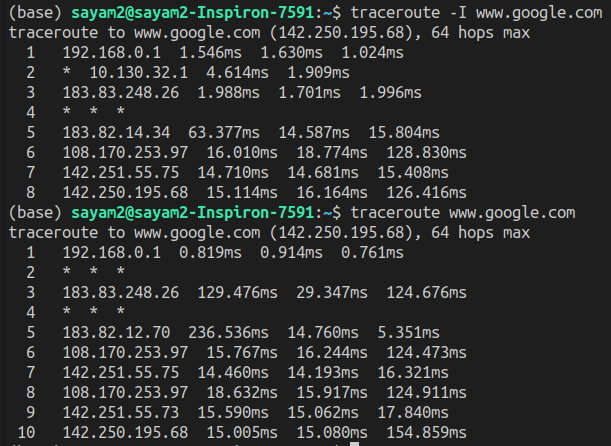
\includegraphics[width=0.5\textwidth]{traceroute_better_google}
            \caption{\texttt{traceroute} with and without \texttt{-I} flag (for \href{https://www.google.com}{Google})}
        \end{figure}
    \item Using the \texttt{-I} flag also permits finding the route for some websites (such as \href{https://www.iitd.ac.in}{IITD}) which is impossible without the flag.
        \begin{figure}[H]
            \centering
            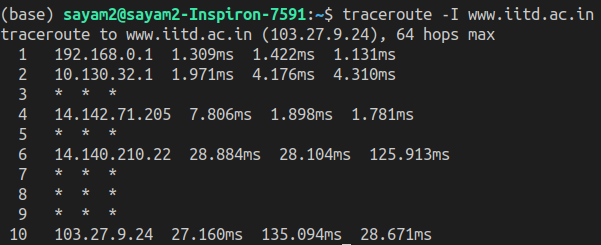
\includegraphics[width=0.5\textwidth]{traceroute_better_iitd}
            \caption{\texttt{traceroute} for \href{https://www.iitd.ac.in}{IITD} with \texttt{-I} flag}
        \end{figure}
    \item To find the best value of the \textit{RTT}, the number of iterations can be increased to establish a stable communication with each router and have a larger success rate of pinging.
\end{enumerate}


\section{Packet Analysis}

\subsection{DNS Filter for \href{http://apache.org}{Apache}}
After the actual DNS query for \url{http://apache.org}, a few DNS queries are made to various Google services (such as YouTube, ad services, etc). These are (mostly) because of the YouTube embeds and other browser/website services. The DNS query for \url{http://apache.org} looks like:
\begin{figure}[H]
    \centering
    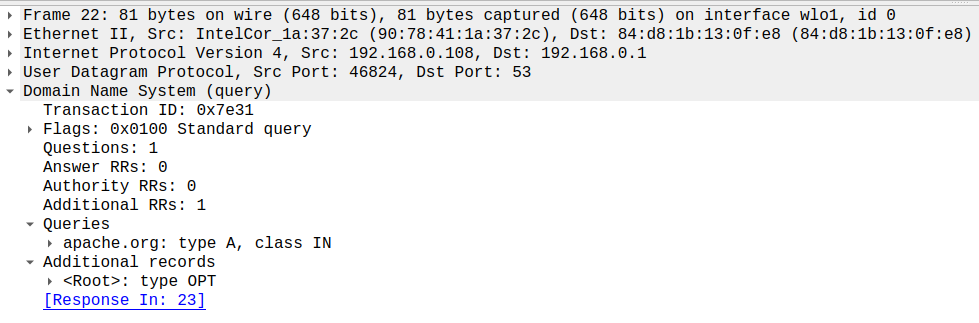
\includegraphics[width=\textwidth]{apache_dns_query}
    \caption{DNS query for \href{http://apache.org}{Apache}}
\end{figure}

The response is received in $68.7$ milliseconds:
\begin{figure}[H]
    \centering
    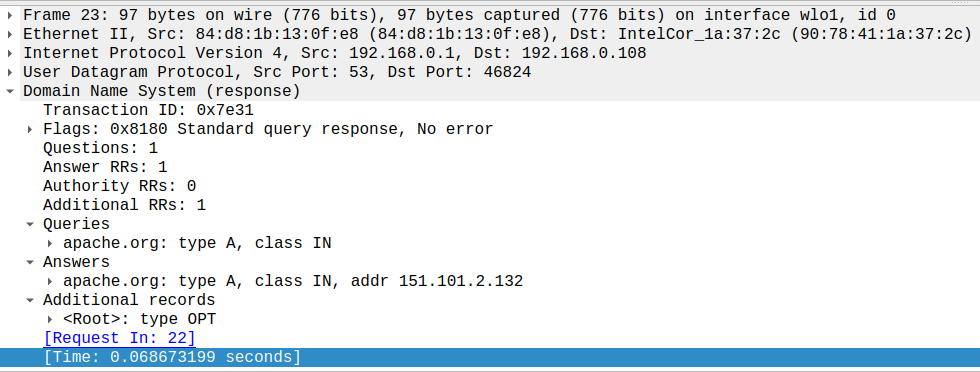
\includegraphics[width=\textwidth]{apache_dns_response}
    \caption{DNS response for \href{http://apache.org}{Apache}}
\end{figure}

\subsection{HTTP Filter for \href{http://apache.org}{Apache}}
$24$ requests were made for the loading of the webpage to the IP address. $6$ additional requests were made to two separate Google IP addresses ($3$ each). The requests were such that each response yielded a single \textit{file} such as:
\begin{itemize}
    \item text/html
    \item text/css
    \item text/javascript (requested from Google)
    \item application/javascript
    \item application/pkix-cert (requested from Google)
    \item font/woff2
    \item PNG
    \item JPEG JFIF image
\end{itemize}
All of the responses yielded a status code of $200$ (except for two responses which were both to Google and they yielded status codes of $204$ and $404$).
\begin{figure}[H]
    \centering
    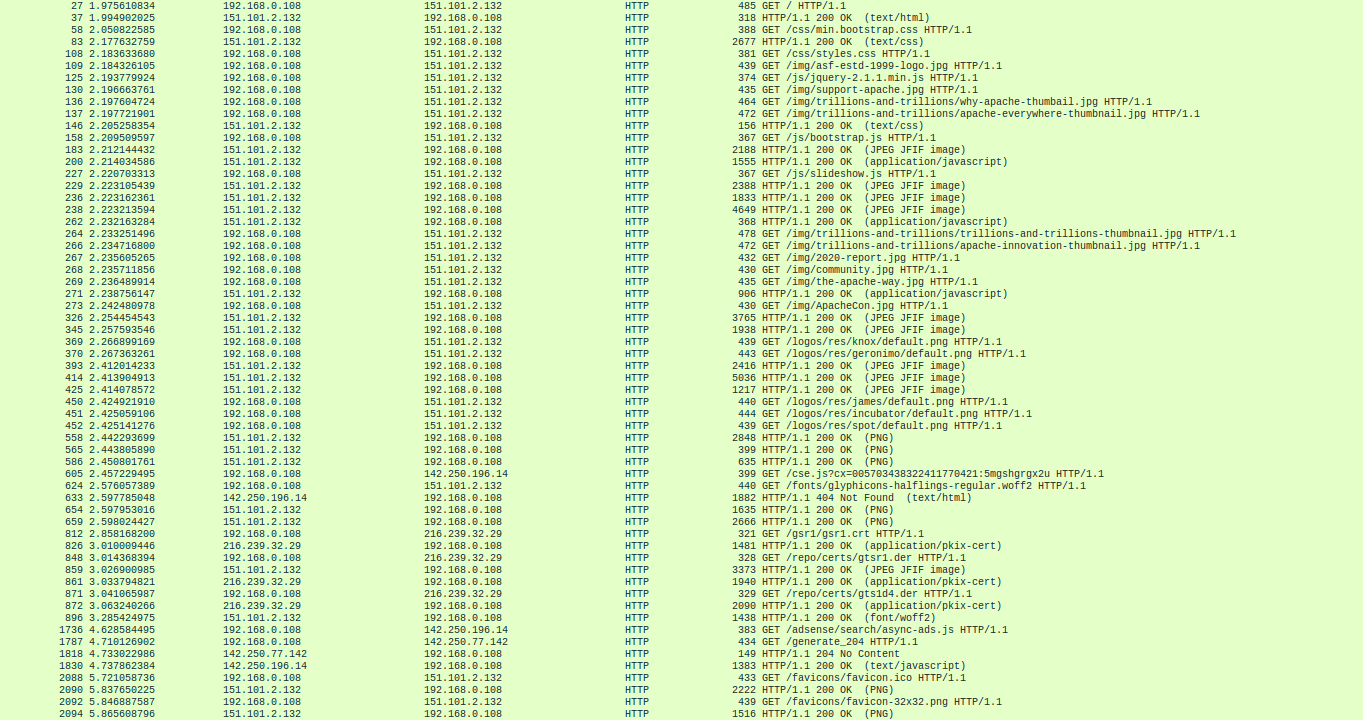
\includegraphics[width=\textwidth]{apache_http}
    \caption{Entire list of HTTP requests and responses for \href{http://apache.org}{Apache}}
\end{figure}

\subsection{Time to Download the Webpage}
The total time taken is defined as:
\[{time}(last\ HTTP\ response) - {time}(first\ DNS\ query)\]
On evaluating, the time is obtained to be $(5.865-1.888)s=\mathbf{3.977s}$

\subsection{HTTP Filter for \href{http://www.cse.iitd.ac.in}{CSE IITD}}
On applying the \textit{HTTP} filter for \url{http://www.cse.iitd.ac.in}, there is a single response with error code $301$, which means that the webpage has been \textbf{Moved Permanently}. The response contains a webpage which \textit{redirects} to \href{https://www.cse.iitd.ac.in}{http\textbf{s}://www.cse.iitd.ac.in}. The communications over \textit{HTTPS} are done over \textbf{TLS} which first includes initiating connection, encryption handshake and
then sharing of information securely.

\begin{figure}[H]
    \centering
    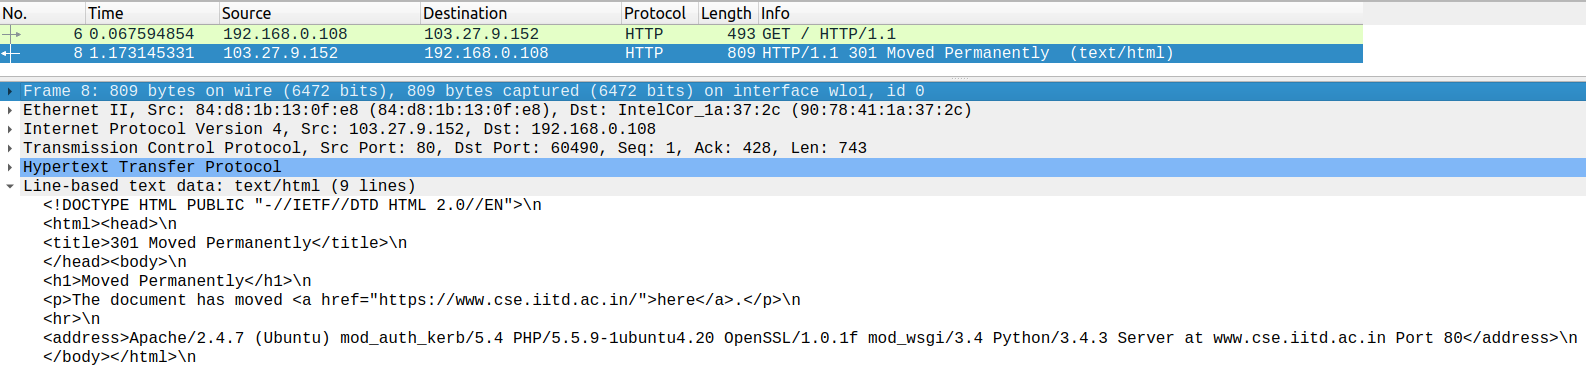
\includegraphics[width=1\textwidth]{cse_http}
    \caption{HTTP request and response for \url{http://www.cse.iitd.ac.in}}
\end{figure}


\section{Implementing Traceroute}

\subsection{Explanation of the Code}
To implement \texttt{traceroute}, socket programming was used to send an \textit{ICMP} echo request (type = $8$) and receive the response from the server setting different hop values. Breaking down the main part of the \texttt{ping} function:\par

\inputminted[firstline=80,lastline=83,bgcolor=mintedbg,linenos]{python}{traceroute.py}
The above code sends the packet and receives it, computing the \textit{RTT} too.\par

\inputminted[firstline=84,lastline=88,bgcolor=mintedbg,linenos]{python}{traceroute.py}
The checksum is verified to be $0$ and then the first byte of the \textbf{header} is analysed. This contains the type of the packet, which equals $0$ on a successful echo and $11$ on TTL exceeded.\par

The remaining code inside the \texttt{ping} function involves setting the \textit{TTL value} and printing relevant information.

\subsection{Working of the Code}

\subsubsection{\href{https://www.github.com}{GitHub}}
\href{https://www.github.com}{GitHub} is used since it has considerable number of hops with routers on the way both responding and not responding. The output and plot of the traceroute looks like:

\inputminted[bgcolor=mintedbg]{text}{outputs/my_traceroute_github}

\begin{figure}[H]
    \centering
    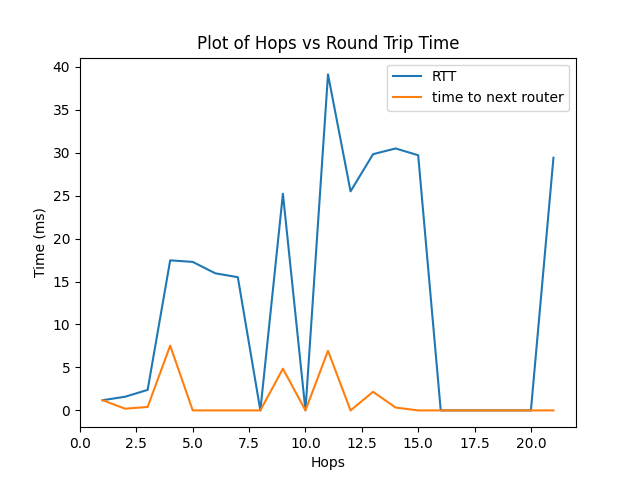
\includegraphics[width=0.66\textwidth]{my_traceroute_github}
    \caption{Plot for \href{https://www.github.com}{GitHub}}
\end{figure}


\subsubsection{\href{https://www.iitd.ac.in}{IITD}}
The output for \href{https://www.iitd.ac.in}{IITD} is also added to the report to show the proper handling of the termination condition, i.e., when the \textit{header type} does not equal \texttt{ICMP echo} even if the returned \textit{IP address} matches (reference to \href{https://piazza.com/class/ksadh5klx166sx?cid=9}{this} Piazza post). The output and plot are as follows:

\inputminted[bgcolor=mintedbg]{text}{outputs/my_traceroute_iitd}

\begin{figure}[H]
    \centering
    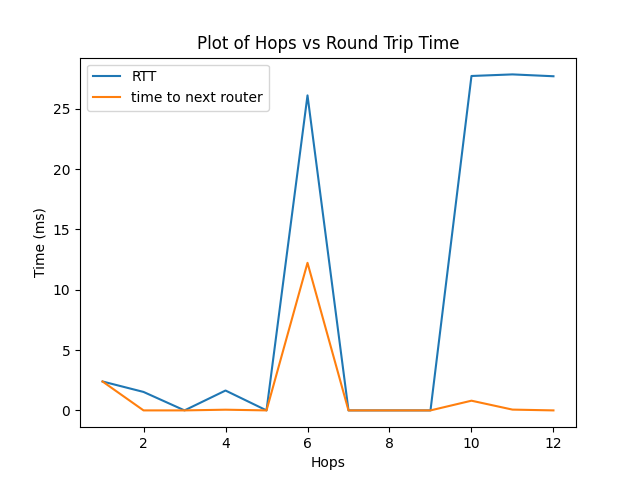
\includegraphics[width=0.66\textwidth]{my_traceroute_iitd}
    \caption{Plot for \href{https://www.iitd.ac.in}{IITD}}
\end{figure}


\end{document}

